\documentclass[10pt]{article}
\usepackage{graphicx}
\usepackage{cases}
\usepackage{fullpage}

\pdfinfo{%
  /Title    (Estimating Spatial Density)
  /Author   (Connor)
  /Creator  (Connor)
  /Producer (Connor)
  /Subject  (Spatial Density)
  /Keywords (PERL GMT spatial density kernel)
}

\begin{document}
\title{Estimating Spatial Density}
\author{Connor - University of South Florida}
\maketitle
Hazard assessments need to rely on robust regional spatial density estimates of the likely occurrence of future hazardous events, such as the location of new volcanic vents or the epicenters of large earthquakes. In volcanology, the distribution of older volcanoes or volcanic vents provides some of the clearest information about the probable location of future volcanoes and volcanic vents (e.g. Crowe~{\it et al.}, 1983; Lutz and Gutmann, 1995; Connor and Hill, 1995; Jaquet and Carniel, 2006; Jaquet~{\it et al.}, 2008). In seismology, historical earthquake catalogs provide information about the probable locations of future large earthquakes (Figure~\ref{fig_eqs}) (e.g. Stirling and Wesnousky, 1998; Musson and Winter, 1996; Stock and Smith, 2002). However, estimating the spatial density of such hazardous events has often proved contentious. Why the controversy? The underlying geologic processes controlling the distribution of these events are complex and incompletely understood. The frequency of such potentially catastrophic events is often low, so data used in these analyses are often sparse. The selection of specific statistical models to estimate spatial density is often subjective. These factors result in uncertainty.

\begin{figure}[!ht]
    \centering
    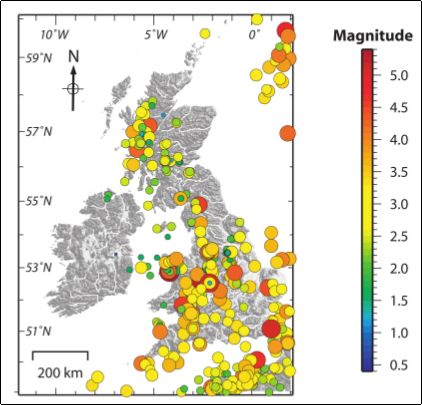
\includegraphics[scale=.60]{figures/UK_equakes.png}
    \caption{Earthquake epicenters are plotted as shaded circles that increase in diameter, proportional to earthquake magnitude. Earthquake catalog data are from the NEIC/USGS database \index{database!earthquake}, Jan.~1973$-$Jan.~2007. These earthquake epicenters, together with a subset found in the ISC catalog, serve as a basis for spatial intensity estimation. Visually, the number of earthquake epicenters decreases west of 7$^\circ$\,W. Topographic data, shown as a shaded relief digital elevation model, is based on 1\,km GLOBE data (GLOBE Task Team, 1999); map datum WGS84.}
    \label{fig_eqs}
\end{figure}
Nonparametric methods, such as kernel density estimation, are efficient and objective estimators of spatial density. In the following, the basis for kernel density estimation is described.

\section{ What is spatial density? }
In the context of volcanic and seismic hazard assessments, the reason for estimating spatial density is to determine possible locations of future geophysical events, or to estimate the probability of an event occurring at a specific location, given that such events occur within the region. Unfortunately, there is some ambiguity in the literature regarding the use of the terms density and intensity. In the geosciences, variation in the number of events per unit area (say the number of volcanic vents or earthquake epicenters) is described using the term density. For example, one might report the density of earthquake epicenters in a region as the number of epicenters per 1000\,km$^2$. Intensity, in geoscience contexts, often refers to the magnitudes of these events. The intensity of ground shaking due to an earthquake can be described with the European macroseimic scale. The intensity of a volcanic eruption can be characterized in terms of its total mass of eruptive products or related indices (Pyle, 2000).

Density and intensity are defined differently in spatial statistics. In this context, spatial intensity refers to the expected number of events per unit area defined at a point, $\bf{s}$, a matrix containing the $x$ and $y$ coordinates of the location of the point (Diggle, 1985; Diggle and Marron, 1988; Gatrell~{\it et al.}, 1996). Suppose there exists a set of events (e.g. earthquake epicenters or volcano locations) that occur within a given region, $R$. These events can be designated as ${\mathbf{x}_n (n=1, 2,...,N)}\in R$ where $N$ is the total number of events, each consisting of the spatial location, $x$ and $y$ of the event (possibly given in Easting and Northing coordinates, or, latitude and longitude). One way we can create a model of spatial intensity from these events is to imagine they are realizations of a random variable, $\bf{X}$, a \index{random variable} function that describes the set of all possible realizations. For example, $\bf{X}$ might be the distribution of potential earthquakes or the distribution of potential volcanoes, from which a set of observed realizations (e.g. those found in the earthquake catalog or on a geologic map) are drawn. The spatial intensity is formally written as (Gatrell~{\it et al.}, 1996)
\begin{equation}
\lambda (\mathbf{s}) = \lim_{d\bf{s} \to 0} \left\{ \frac{E(\bf{X})}{d\bf{s}} \right\}
\label{eq14-1}
\end{equation}
where $E(\bf{X})$  is the expected number of events that fall within a small area $d\bf{s}$ about the point $\bf{s}$ (hence, if the location, $\bf{s}$, is given as Easting and Northing with units of meters, then the units of $\lambda(\bf{s})$ are m$^{-2}$). At first glance it appears that the statistical definition of {\it intensity} is equivalent to the term {\it density} as commonly used in the geosciences. This is not quite true. The geological processes that result in a given event distribution are incompletely known. We can think of these geological processes as giving rise to a stochastic point process that describes the relationship between the set of events and the geological processes that led to their formation. As the stochastic point process is incompletely known, the true value of the local spatial intensity, $\lambda(\bf{s})$, is also unknown. That is, the observed distribution of events is only one realization of the underlying process that gives rise to these events. Our goals are to find an estimate of the spatial intensity, $\hat\lambda(\bf{s})$, that approximates the true but unknown value of spatial intensity, $\lambda(\bf{s})$, and to understand the uncertainty in this estimate.

In hazard assessments, there is a further requirement, that this information be used to forecast the spatial distribution of possible future events. Often we consider spatial intensity in terms of the probable location of some future event, given that one occurs within our region of interest. This conditional probability can be estimated by:
\begin{equation}
\hat f (\mathbf{s}) = \frac{\hat\lambda(\mathbf{s})}{\int_R \hat\lambda(\mathbf{s})d(\mathbf{s})}.
\label{eq14-2}
\end{equation}
Integrating $\hat f(\bf{s})$ across the region of interest, $R$, gives unity, if $R$ is sufficiently large. Since all values of $\hat f(\bf{s})$ within this region are greater than or equal to zero, this makes $\hat f(\bf{s})$ a probability density function and this function may be used in probabilistic hazard models. $\hat f(\bf{s})$ is referred to as one estimate of the spatial density, and one can consider the spatial density per unit area in terms of conditional probability (e.g. given a volcanic event in the region, what is the probability that the event will occur within some small area about the point $\mathbf{s}$?). In addition, care is required in the selection of the region $R$, as external events located close to the border may have a non-negligible contribution to spatial density. A practical approach is to select $R$ to be quite large compared to the region of specific interest (e.g. the volcanic system). In the following, we refer to spatial intensity and spatial density within the context of spatial statistics.

\section{ Assumptions behind spatial density estimates }
How does one develop a best estimate of spatial density? In the real world, there is only one realization of an underlying geologic process, the observed distribution of past events. Unfortunately, geology is not conducive to repeating the experiment in a natural system. For a given region there is just one earthquake catalog, or one geologic map of volcano distribution. Presumably, if there existed a complete geophysical model for these events, we would use this information to better forecast the locations of future events. For example, if we knew the distribution of melt in the asthenosphere and lithosphere, and if we knew the state of the lithosphere through which the magma rises, we might have a better sense of where volcanoes or volcanic vents are most likely to form next. Currently, we lack such a complete geophysical perspective. Some data sets give an idea of where partial melting of the mantle might occur, for example seismic tomographic models of ``slowness'' in the lithosphere and asthenosphere (e.g. Zhao, 2001). Other data, such as variations in gravity across a region (Connor~{\it et al.}, 2000; Parsons~{\it et al.}, 2006), show some correlation with the existing distribution of volcanoes in some circumstances, but the mechanisms relating gravity anomalies to the origin of magmas are not completely understood. As a result, these types of data have been used to support estimates of spatial density (e.g. Connor~{\it et al.}, 2000; Martin~{\it et al.}, 2004), but no model has yet been proposed that does not rely principally on the spatial distribution of past events. Similarly, in seismology there have been attempts to create blended hazard maps \index{hazard map} based on a variety of geophysical criteria, but these methods generally rely on the earthquake catalog (e.g. Ward, 1994). 

The reliance on the distribution of past events implies that these realizations are representations of some underlying random variable, $\bf{X}$, that will govern the distribution of potential events in the future. This assumption immediately raises a fundamental question. Which are the past events that should be used to develop the spatial intensity estimate, $\hat\lambda(\bf{s})$ , and density, $\hat f(\bf{s})$? Event datasets used to estimate the spatial density of future events need to be consistent with several features of geological processes.

First, any spatial intensity function for a geologic process must change with time. On time scales of tens of millions of years, plate boundaries change, volcanic arcs wax, wane, and migrate, and major fault systems reorganize. In very long term probabilistic hazard assessments for high-level waste repositories, which may have 10$^6$\,a performance periods, these factors have to be considered in weighing the validity of using specific data in developing spatial intensity models. For processes like volcanism, where a geologic record of past events usually persists for tens of millions of years, consideration needs to be given to which events best represent the distribution of future volcanism. For example, the distribution of Miocene volcanoes in a given area might be much less relevant than the distribution of Pliocene and Quaternary volcanoes. Thus, in order to develop an estimate of the spatial intensity, a model of the geologic evolution of the system is required. This geological model is used to justify the inclusion of some geological features in the event dataset, and the exclusion of others.

Second, it is necessary to assess the completeness of the geologic record. In seismology, it is particularly clear that short earthquake catalogs carry the risk of biasing estimates of spatial intensity. That is, the record of earthquakes in a given region collected on a short time scale might give an incomplete picture of the unknown distribution of potential earthquakes, $\lambda(\bf{s})$. Even volcanic events might be missed in initial geological investigations, as volcanic vents might be buried in sediment or otherwise obscured (e.g. Connor~{\it et al.}, 1997; Wetmore~{\it et al.}, 2009).

Third, geological events, even when they are all identified, may be so rare as to present an incomplete picture of the underlying process. Consider an earthquake as a single event, $\mathbf{x}_n$, one realization of the random variable, $\bf{X}$. If, for example, $\bf{X}$ can be characterized by a uniform random distribution, then it is likely that the observed set of realizations will have a spatially random distribution within the region of interest, $R$. However, the underlying density usually has additional structure, causing independent realizations to cluster. For example, earthquake epicenters tend to cluster along plate boundaries and volcanoes cluster above zones of partial melting in the mantle. For random variables with a great deal of statistical structure, such as many modes in spatial intensity, a great number of events might be required to identify the statistical structure of the random variable.

Fourth, it is critical to ascertain which geologic features are actually independent events. The true statistical structure of the random variable, $\bf{X}$, might be obscured if some events included in the event dataset are not independent.  For example, great earthquakes are followed by aftershocks. An earthquake aftershock, however, is not a random sample of the random variable ``{\it spatial distribution of great earthquakes}'', because these aftershocks are not realizations of this particular random variable. Rather, they are independent realizations of another random variable, say ``{\it spatial distribution of aftershocks about a great earthquake}''. So, the distribution of aftershocks does not necessarily give the best sense of the spatial intensity of great earthquakes, although these two random variables are correlated.

Similarly, volcanoes are complex geologic structures. The spatial distribution of polygenetic volcanoes reflects processes of magma generation and rise through the crust. The distribution of small vents (sometimes referred to as parasitic or adventive cones) does not necessarily reflect the distribution of polygenetic volcanoes, so a spatial intensity estimate that includes all vents as events would not correctly model the underlying random variable. Furthermore, in monogenetic volcanic fields  alignments of volcanic cones develop in response to single magmatic events,  episodes of magma rise through the shallow crust. This is because single igneous dikes ascending through the crust might form segments and rotate within the shallow crust, each segment feeding a separate vent and each building a volcanic cone.  If the goal of analysis is to forecast the distribution of future magmatic events, each of which might produce more than one monogenetic volcano, geological data must be gathered and volcanoes formed by the same magmatic event must be somehow grouped as single events.

Independence of events is not necessarily easy to determine. Rather than simply counting earthquakes in a catalog or volcanoes on a geologic map, one must make a geologic assessment of the independence of these data. For volcanoes, this is generally accomplished through detailed analyses of radiometric age determinations, stratigraphic correlations, and related geologic data. Often, even detailed analyses do not resolve whether or not specific features should be grouped as single events or treated as separate, independent events.

Consequently, a major task in preparing a spatial intensity estimate is defining the dataset of events to be used. Certainly a major expense in hazard assessment for a community is data gathering to support interpretation of geological features as events. Mahoney~{\it et al.} 2009) and Stirling~{\it et al.} (2009) provide examples of such analyses. Hazard assessments often consider alternative event datasets and account for the affect of these varying datasets on spatial density estimates. This strategy will be employed in the following examples.

\section{Estimating spatial intensity with kernel methods}
Spatial intensity models based on the distribution of past volcanic or seismic events might be parametric or nonparametric. Parametric models involve fitting a distribution, usually one from a common set of distributions (e.g. uniform random or bivariate Gaussian) to the distribution of events throughout a region or within zones (i.e. subsets of the region of interest). This estimate yields a set of parameters (e.g. mean location of the volcanic field in Northing and Easting coordinates, variance in Northing and Easting coordinates, or rotation). Uncertainty in the distribution fit, and uncertainty in parameter estimates of spatial intensity, can be calculated using maximum likelihood estimation. A significant drawback of these parametric methods is that they assume {\it a priori} that the distribution of volcanoes is explained by the parametric distribution, for example that volcano distribution is reasonably described as a bivariate Gaussian density. This is not necessarily the case. In fact, it has been shown repeatedly that volcanoes cluster within volcanic fields. Such clustering may be completely smoothed by simple parametric models. To our knowledge, parametric models have not been used to model earthquake intensity, although completely spatially random models within zones are parametric in the most general sense (Beauval1~{\it et al.}, 2006).

A nonparametric approach for estimating the spatial intensity involves kernel density estimation (Silverman, 1978; Diggle, 1985; Silverman, 1986; Wand and Jones, 1995). With this technique, the observed event locations are used to estimate the spatial intensity at any point in the region using a kernel function. For example,
\begin{equation}
\hat\lambda (\mathbf{s}) = \frac{1}{2\pi h^2}\sum^N_{i=1} \exp \left[ -\frac{1}{2} \left(\frac{d_i}{h}\right)^2 \right]
\label{eq14-3}
\end{equation}
is a 2D radially-symmetric kernel function where the spatial intensity decreases with distance from events based on a bivariate Gaussian function. The local spatial intensity estimate, $\hat\lambda(\bf{s})$, depends on its distance, $d_i$, to each event location, and the smoothing bandwidth, $h$. The rate of change in spatial intensity with distance from events depends on the size of the bandwidth, which, in the case of a Gaussian kernel function, is equivalent to the standard deviation of the kernel. In this example, the kernel is radially symmetric, that is, $h$ is constant in all directions. Nearly all kernel estimators used in geologic hazard assessments have been of this type (e.g. Woo, 1996; Stock and Smith, 2002; Connor and Hill, 1995; Condit and Connor, 1996). The bandwidth is selected using some criterion, often visual smoothness of the resulting spatial intensity plots, and the spatial intensity function is calculated using this bandwidth. Alternatively, an adaptive kernel function can be used, in which the spatial intensity varies as a function of event spatial intensity (e.g. Stock and Smith, 2002; Weller~{\it et al.}, 2006). These adaptive kernel functions are also radially symmetric.

Here is a snippet of PERL code that illustrates the implmentation of equation (\ref{eq14-3}) in code:
\begin{verbatim}
 $sumn=0;
 for ($i=0; $i<$N; $i++) {
      # here is the distance squared formula
      $dist1=($x-$volcanoes[$i][0])*($x-$volcanoes[$i][0]) 
           + ($y-$volcanoes[$i][1])*($y-$volcanoes[$i][1]);

      #now calculate and sum the kernel
      $dist2 = $dist1/($h*$h);
      $kuu = 1/(2*3.14159) * exp(-0.5*$dist2);
      $sumn += 1.0/($h*$h) * $kuu;
 }
\end{verbatim}

Note that $h$ has to be specified elsewhere in the code, the array $volcanoes$ contains the spatial information (Easting, Northing) about the point distribution, and $N$ is the total number of volcanoes in the dataset for which spatial density is estimated. In this code, spatial density is estimated at the point $x, y$. If there are many such points (say the calculation is done on a grid, then this snippet of code must be executed repeatedly.

Equation (\ref{eq14-3}) is a simplification of the more general case, whereby the amount of smoothing by the bandwidth, $h$, varies in magnitude depending on direction. A two-dimensional elliptical kernel with a direction varying bandwidth is given by (Wand and Jones, 1995),
\begin{equation}
\hat\lambda (\mathbf{s}) = \frac{1}{2\pi \sqrt{|\bf{H}|}} \sum^N_{i=1} \exp \left[ -\frac{1}{2}\bf{b}^T \bf{b}\right]
\label{eq14-4}
\end{equation}
where,
\begin{equation}
\bf{b}=H^{-1/2}\bf{d}.
\label{eq14-5}
\end{equation}
The bandwidth, $\bf{H}$, is a $2\,\times\,2$ element matrix \index{kernel!bandwidth matrix} that is positive and definite (important because the matrix must have a square root), $|\bf{H}|$ is the determinant of this matrix and $\bf{H}^{-1/2}$ is the inverse of its square root. $\bf{d}$ is a $1\,\times\,2$ distance matrix (i.e. the $x$-distance and $y$-distance from $\bf{s}$ to an event), $\bf{b}$ is the cross product of $\bf{d}$ and $\bf{H}^{-1/2}$, and $\bf{b}^T$ is its transform. The resulting spatial intensity at each point location, $\bf{s}$, is usually distributed on a grid which has total extent that defines the region, $R$.

One difficulty with elliptical kernels is that all elements of the bandwidth matrix must be estimated. Several methods have been developed for estimating an optimal bandwidth matrix based on the locations of the event data (Wand and Jones, 1995), most recently summarized in the statistics literature by Duong~(2007). Here we utilize two techniques, a modified asymptotic mean integrated squared error (AMISE) method, developed by Duong and Hazelton (2003), called the SAMSE pilot bandwidth \index{pilot bandwidth} selector, and the smoothed cross-validation (SCV) method of Hall~{\it et al.} (1992), to optimally estimate the smoothing bandwidth for our Gaussian kernel function. These bandwidth estimators are found in the freely-available $R$~statistical package (Hornik, 2007; Duong, 2007). \index{$R$~statistical package}

\section{Uncertainty in spatial density estimates}
\index{uncertainty} Uncertainty exists in the estimates of spatial density. This uncertainty stems from: {\it (i)} ambiguity in event data sets used to develop kernel estimates, {\it (ii)} application of the kernel density function, {\it (iii)} uncertainty in the bandwidth estimate used in the kernel density estimation, and {\it (iv)} few event data, a common problem in hazard assessment. Each of these in considered in the following, with particular emphasis on the treatment of uncertainty arising from sparse data.

\subsection{Event definition}
Event definition affects the total number of events used to estimate density, and may introduce bias in density estimates. This tends to diminish the weight associated with events in the center of the distribution in this particular case, as these events all formed multiple volcanoes See Wetmore~{\it et al.} (2009) for an additional example of a spatial density estimation of volcanism that is changed by including additional evidence of volcanism from subsurface investigations.

\subsection{Kernels functions}
Spatial density estimates made using kernel functions, as opposed to hazard zonation models (e.g. Crowe~{\it et al.}, 1983; Musson, 1997) or parametric models, are explicitly data driven. A basic advantage of this approach is that any spatial density estimate will be consistent with the known data. Equations (\ref{eq14-3}) and (\ref{eq14-4}) are bivariate Gaussian kernels. Numerous authors have shown that the use of other kernels, such as the Epanechnikov kernel \index{Epanechnikov kernel function} (Connor and Hill, 1995) or the Cauchy kernel (Martin~{\it et al.}, 2004) \index{Cauchy kernel function} has little impact on the final density estimate (e.g. Silverman, 1986; Wand and Jones, 1995). In hazard assessment, kernel functions with infinite tails (e.g. Gaussian) are preferred, as the probability is positive and real everywhere, albeit very small at locations far from past events. A picture of a kernel function, contoured around a single point, is shown in Figure~\ref{fig_kernel}. A potential disadvantage of these kernel functions is that they are not inherently sensitive to geologic boundaries. One might hope that a complete understanding of the geology would result in a modification of the density estimate derived from a mathematical function. In fact, Connor~{\it et al.} (2000) and Martin~{\it et al.} (2004) discuss various methods of weighting density estimates in light of geological or geophysical information, in a manner similar to Ward (1994). A difficulty with such weighting is the subjectivity involved in recasting geologic observations as density functions. Furthermore, geologic insight is not always consistent with event distributions. For example, Musson (1997) noted, with some frustration, that epicenter distribution in the UK does not correlate well or consistently with known major geologic structures that would be expected from a geophysical perspective to host earthquakes. Thus, even if a zonation model is used in hazard assessments, it makes sense to calculate the kernel-based density estimates and to consider any discrepancies in these models explicitly.


\begin{figure}[!ht]
    \centering
    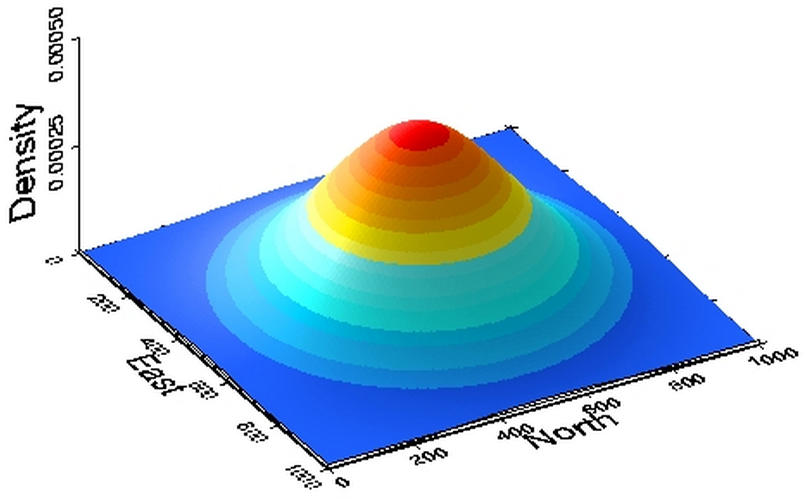
\includegraphics[scale=.30]{figures/kernel.png}
    \caption{Shaded-relief map of a Gaussian kernel function drawn about a single point. The point is located at the highest spatial density.}
    \label{fig_kernel}
\end{figure}

\subsection{Kernel bandwidth}
Bandwidth selection is a key feature of kernel density estimation, and is particularly relevant to seismic and volcanic hazard studies (e.g. Stock and Smith, 2002; Connor~{\it et al.}, 2000; Molina~{\it et al.}, 2001; Abrahamson, 2006;  Jaquet~{\it et al.}, 2008).  Bandwidths that are narrow focus density near past events. Conversely, a large bandwidth may over-smooth the density estimate, resulting in unreasonably low density estimates near clusters of past events, and overestimate density far from past events. This dependence on bandwidth can create ambiguity in the interpretation of spatial density if bandwidths are arbitrarily selected (Abrahamson, 2006).

 Bivariate bandwidth selectors like the SCV and SAMSE methods appear to be very promising, because although they are mathematically complex, they find optimal bandwidths using the actual data locations, removing subjectivity from the process. The bandwidth selectors used in this chapter provide global estimates of density, in the sense that one bandwidth or bandwidth matrix is used to describe variation across the entire region. An alternative method is to use adaptive kernel estimates, in which case the bandwidth changes with event density (Stock and Smith, 2002; Weller~{\it et al.}, 2006). These adaptive bandwidths are calculated assuming radially symmetric kernel functions. Future research will likely involve developing bandwidth selectors that are adaptive across the map region.

\subsection{Sparse event data}
Often in hazard assessment there is a ``problem'' that there are few data available from which to forecast future events. That is, often hazard assessments are needed for places where events are not so frequent that the geologic hazards are completely obvious. Instead, hazard analysis is most often required were few geologically hazardous events have occurred in the past. This is paradoxical because, by definition, uncertainty in hazard assessments must be comparatively high in these regions. If a spatial density is estimated using thousands of earthquakes or hundreds of volcanoes, we can assume that the true density is well-represented by this model. Conversely, if the spatial intensity estimate is based on a handful of events, we might expect high uncertainty in the estimate. For example, the discovery of a single additional volcano, buried in sediment, might alter the shape of the estimated regional spatial density.

An example of a spatial density map is shown in Figure~\ref{UK_kernel}, for the largest earthquakes to have occured in recent years in the UK. Note that different assumptions (in this case different kernel bandwidths) produce slightly different models (and maps) of earthquake spatial density. How would you assess this effect in a hazard assessment?

\begin{figure}
\centering
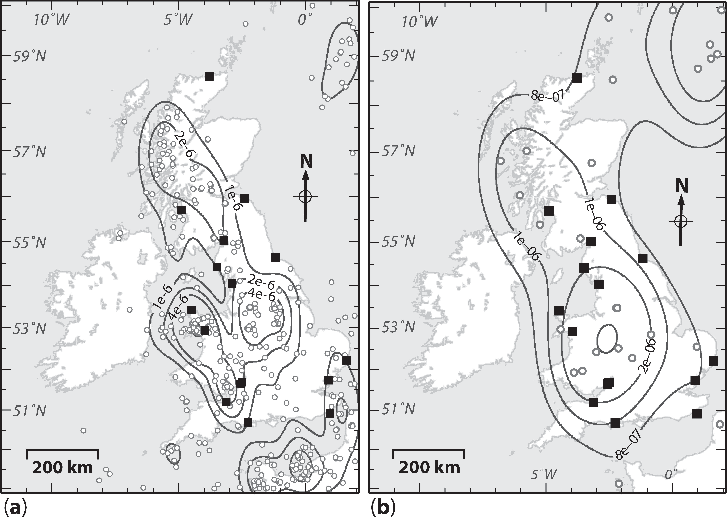
\includegraphics{./figures/UK_kernel.pdf}
\caption{Map (a) shows the regional spatial density estimate based on all earthquakes, including aftershocks, from Jan., 1973$-$Jan., 2007, based on the NEIC catalog. Map (b) includes only those earthquake events of magnitude $> 3$\,ML, based on the ISC catalog. Both spatial density maps use bandwidths chosen by the SAMSE method.  The maps are contoured at the 1$^{st}$, 25$^{th}$, 50$^{th}$, and 75$^{th}$ spatial density percentiles. As an example, using map (b), locations within the 1e-06 (75$^{th}$ percentile) contour have a spatial density greater than 1$\times 10^{-6}$ per 100\,km$^2$, or 1$\times 10^{-8}$\,km$^{-2}$. The smoother density map (b) may better reflect the true potential distribution of larger earthquakes since aftershocks are not included in this estimate. The black squares represent the locations of nuclear facilities. Are some nuclear facilitites located in more earthquake prone areas than others?}
\label{UK_kernel}
\end{figure}
\begin{thebibliography}{99}
\small{
\bibitem{14abr}
Abrahamson, N. (2006). Seismic hazard assessment: Problems with current practice and future developments. Presented at 1$^{st}$ European Conference on Earthquake Engineering and Seismology, Geneva, Switzerland, 3$-$8 September, keynote address.

\bibitem{14bea}
Beauval1, C., S. Hainzl and F. Scherbaum (2006). The impact of the spatial uniform distribution of seismicity on probabilistic seismic-hazard estimation. {\it Bulletin of the Seismological Society of America},  {\bf96}, 2465$-$2471, doi:10.1785/0120060073.

\bibitem{cond}
Condit, C. D. and C. B. Connor (1996). Recurrence rate of basaltic volcanism in volcanic fields: An example from the Springerville Volcanic Field, AZ, USA. {\it Geological Society of America, Bulletin}, {\bf 108}, 1225$-$1241.

\bibitem{14con}
Connor, C. B. and B. E. Hill 1995. Three nonhomogeneous Poisson models for the probability of basaltic volcanism: Application to the Yucca Mountain region. {\it Journal of Geophysical Research}, {\bf 100}, 10\,107$-$10\,125.

\bibitem{14con1}
Connor, C. B., S. Magsino and J. Stamatakos {\it et al.} (1997). Magnetic surveys help reassess volcanic hazards at Yucca Mountain. {\it Eos, Transactions of the American Geophysical Union}, {\bf 78}(7), 73,77$-$78.

\bibitem{14con2}
Connor, C. B., J. Stamatakos, D. Ferrill, B. E. Hill, G. Ofoegbu and F. M. Conway (2000). Volcanic hazards at the proposed Yucca Mountain, Nevada, high-level radioactive waste repository. {\it Journal of Geophysical Research}, {\bf 105}, 417$-$432.

\bibitem{cop}
Coppersmith, K. J. and R. R. Youngs (1986). Capturing uncertainty in probabilistic seismic hazard assessments within intraplate tectonic environments. {\it Proceedings of the Third U.S. National Conference on Earthquake Engineering, Charleston}, {\bf 1}, 301$-$312.

\bibitem{14cro}
Crowe, B. M., D. T. Vaniman and W. J. Carr (1983). Status of volcanic hazard studies for the Nevada nuclear waste storage investigations, Lab Report {\bf LA-9325-MS}. Los Alamos National Lab, NM.

\bibitem{dig}
Diggle, P. (1985). A kernel method for smoothing point process data. {\it  Applied Statistics}, {\bf 34}, 138$-$147.

\bibitem{dig1}
Diggle, P. and J. S. Marron (1988). Equivalence of smoothing parameter selectors in density and intensity estimation. {\it Journal of the American Statistical Association}, {\bf 83}, 793$-$800.

\bibitem{duo}
Duong, T. (2007). ks: Kernel Density Estimation and Kernel Discriminant Analysis for Multivariate Data in R. {\it Journal of Statistical Software}, {\bf 21}(7), 1$-$16.

\bibitem{duo1}
Duong, T. and M. L. Hazaelton (2003). Plug-in bandwidth selectors for bivariate kernel density estimation. {\it Journal of Nonparametric Statistics}, {\bf 15}, 17$-$30.

\bibitem{14efr}
Efron, B. and R. Tibishrani (1991). Statistical data analysis in the computer age. {\it Science}, {\bf 253}, 390$-$394.

\bibitem{gat}
Gatrell, A. C., T. C. Bailey, P. J. Diggle and B. S. Rowlingson (1996). Spatial point pattern analysis and its application in geographical epidemiology. {\it Transactions - Institute of British Geographers} {\bf 21}(1), 256$-$274.

\bibitem{glo}
GLOBE Task Team and others (Hastings, David A., Paula K. Dunbar, Gerald M. Elphingstone, Mark Bootz, Hiroshi Murakami, Hiroshi Maruyama, Hiroshi Masaharu, Peter Holland, John Payne, Nevin A. Bryant, Thomas L. Logan, J.-P. Muller, Gunter Schreier, and John S. MacDonald) (eds) (1999). {\it The Global Land One-kilometer Base Elevation (GLOBE) Digital Elevation Model}, Version 1.0. National Oceanic and Atmospheric Administration, National Geophysical Data Center, 325 Broadway, Boulder, Colorado 80303, U.S.A. Digital data base on the World Wide Web (URL: http://www.ngdc.noaa.gov/mgg/topo/globe.html) and CD-ROMs.

\bibitem{hal}
Hall, P., J. S. Marron and B. U. Park (1992). Smoothed cross-validation. {\it Probability Theory and Related Fields}, {\bf 92}, 1$-$20.

\bibitem{hor}
Hornik, K. (2007).  The R-FAQ, http://www.r-project.org/, ISBN 3-900051-08-9.

\bibitem{14int}
ISC (2007). On-line Bulletin, http://www.isc.ac.uk, International  Seismology Centre, Thatcham, United Kingdom.

\bibitem{neic}
NEIC/USGS (2007). On-line EQ database, http://neic.usgs.gov/neis/epic/epic.html, USGS National Earthquake Information Center, US Geological Survey, Reston, VA.

\bibitem{jaq}
Jaquet, O. and R. Carniel (2006).  Estimation of volcanic hazards using geostatistical methods. {\it In}: H. M. Mader {\it et al.} (eds), {\it Statistics in Volcanology}, Special Publications of IAVCEI {\bf 1}. London: Geological Society, 77$-$87.

\bibitem{jaq1}
Jaquet, O., C. B. Connor and L. Connor (2008). Long-term volcanic hazard assessments for nuclear facilities. {\it Nuclear Technology}, {\bf 163}, 180$-$189.

\bibitem{jar}
Jarvis A., H. I. Reuter, A. Nelson and E. Guevara (2006). Hole-filled seamless SRTM data V3, International Centre for Tropical Agriculture (CIAT), available from http://srtm.csi.cgiar.org.

\bibitem{lut}
Lutz, T. M. and J. T. Gutmann (1995). An improved method for determining alignments of point-like features and its implications for the Pinacate volcanic field, Sonora, Mexico. {\it Journal of Geophysical Research}, {\bf 100}, 17\,659$-$17\,670.

\bibitem{14mar}
Martin, A. J., K. Umeda, C. B. Connor, J. N. Weller, D. Zhao and M. Takahashi (2004). Modeling long-term volcanic hazards through Bayesian inference: example from the Tohoku volcanic arc, Japan. {\it Journal of Geophysical Research}, {\bf 109}, B10208, DOI:10.1029/2004JB003201.

\bibitem{mol}
Molina, S., C. D. Lindholm and H. Bungum (2001). Probabilistic seismic hazard analysis: zoning free versus zoning methodology, Bollettino di Geofisica Teorica et Applicata. {\bf 42}(1-2), 19$-$39.

\bibitem{14mus}
Musson, R. M. W. (1997). Seismic hazard studies in the UK: source specification problems of intraplate seismicity. {\it Natural Hazards}, {\bf 15}, 105$-$119.

\bibitem{14mus1}
Musson, R. M. W. and P. W. Winter  (1996). Seismic hazard maps of the UK. {\it Natural Hazards}, {\bf 14}(2$-$3), 141$-$154.

\bibitem{par}
Parsons, T., G. A. Thompson and A. H. Cogbill (2006). Earthquake and volcano clustering via stress transfer at Yucca Mountain, Nevada. {\it Geology}, {\bf 34}, 785$-$788, doi:10.1130/G22636.1.

\bibitem{pre}
Press, W. H., B. P. Flannery, S. A. Teukolsky and W. T., Vetterling (1992). {\it Numerical Recipes in C}, 2nd ed. Cambridge: Cambridge University Press.

\bibitem{14pyl}
Pyle, D. M. (2000). Sizes of volcanic eruptions. {\it In}: H. Sigurdsson {\it et al.} (eds), {\it Encyclopedia of Volcanoes}. New York: Academic Press, 263$-$271.

\bibitem{sil}
Silverman, B.W. (1978). Choosing the window width when estimating a density. {\it Biometrika}, {\bf 65}, 1$-$11.

\bibitem{sil1}
Silverman, B. W. (1986). Density Estimation for Statistics and Data Analysis. {\it Monographs on Statistics and Applied Probability} {\bf 26}. London: Chapman and Hall.

\bibitem{14smi}
Smith, E. I., S. Morikawa and A. Sanchez (1997). Volcanism Studies Related to the Probabilistic Volcanic Hazard at Yucca Mountain for the Period 1986$-$1996, University of Nevada, Las Vegas, http://www.state.nv.us/nucwaste/yucca/volcan01.htm.

\bibitem{14sti}
Stirling, M. and S. G. Wesnousky (1998). Comparison of Recent Probabilistic Seismic Hazard Maps for Southern California. {\it Bulletin of the Seismological Society of America}, {\bf 88}, 855$-$861.

\bibitem{14sto}
Stock, C. and E. G. C. Smith (2002). Comparison of Seismicity Models Generated by Different Kernel Estimations. {\it Bulletin of the Seismological Society of America}, {\bf 92}, 913$-$922.

\bibitem{val}
Valentine, G.A. and F.V. Perry (2007). Tectonically controlled, time-predictable basaltic volcanism from a lithospheric mantle source (central Basin and Range Province, USA). {\it Earth and Planetary Science Letters}, {\bf 261}, 201$-$216.

\bibitem{wan}
Wand, M.P. and M.C. Jones (1995). Kernel Smoothing. {\it Monographs on Statistics and Applied Probability} {\bf 60}. London: Chapman Hall.

\bibitem{14war}
Ward, S. N. (1994). A multidisciplinary approach to seismic hazard in southern California. {\it Bulletin of the Seismological Society of America}, {\bf 84}, 1293$-$1309.

\bibitem{14wel}
Weller, J. N., A. W. Martin, C. B. Connor, L. Connor and A. Karakhanian (2006). Modelling the spatial distribution of volcanoes: an example from Armenia. {/it In:} H. M. Mader {\it et al.} (eds), {\it Statistics in Volcanology}, Special Publications of IAVCEI {\bf 1}. London: Geological Society, 77$-$87.

\bibitem{wes}
Wessel, P. and W. H. F. Smith (1991). Free software helps map and display data. {\it EOS, Transactions of the American Geophysical Union}, {\bf 72}, 441.

\bibitem{woo}
Woo, G. (1996). Kernel estimation methods for seismic hazard area source modelling. {\it Bulletin of the Seismological Society of America},  {\bf 86}, 353$-$362.

\bibitem{14yog}
Yogodzinski, G. M., T. R. Naumann, E. I. Smith and T. R. Bradshaw (1996). Evolution of a mafic volcanic field in the central Great Basin,
south central Nevada. {\it Journal of Geophysical Research}, {\bf 101}, 17\,425$-$17\,445.

\bibitem{14zha}
Zhao, D. (2001). Seismological structure of subduction zones and its implications for arc magmatism and dynamics. {\it Physics of the Earth and Planetary Interiors}, {\bf 127}, 197$-$214.

}
\end{thebibliography}
\end{document}

